\begin{example}[Determinant]
\ \begin{itemize}
	\item[] \textbf{[ Two Categories ]}
	\begin{enumerate}
		\item \textbf{Category of Commutative Rings} ($\mathsf{CRing}$)
		\begin{itemize}
			\item \textbf{Objects}: Commutative rings $R,S,...$
			\item \textbf{Morphisms}: Ring homomorphisms $\phi:R\to S$
		\end{itemize}
		\item \textbf{Category of Groups} ($\mathsf{Grp}$)
		\begin{itemize}
			\item \textbf{Objects}: Groups
			\item \textbf{Morphisms}: Group homomorphisms
		\end{itemize}
	\end{enumerate}
	\item[] \textbf{[ Two Functors ]} Note that $\mathbf{GL}_n$ represents the functor, while $GL_n$ denotes the group.
	\begin{enumerate}
		\item \textbf{General Linear Group Functor} ($\mathbf{GL}_n:\mathsf{CRing}\to\mathsf{Grp}$)
		\begin{itemize}
			\item \textbf{On Objects}: \[
			R\mapsto GL_n(R)
			\] Maps a ring $R$ to the general linear group $GL_n(R)$, which consists of all $n\times n$ invertible matrices over $R$.
			\item \textbf{On Morphisms}: Let $\mathbf{GL}_n(\phi):GL_n(R)\to GL_n(S)$. \[
			\phi\mapsto\mathbf{GL}_n(\phi)
			\] It preserves invertibility.
		\end{itemize}
		\item \textbf{Unit Functor} ($\mathbf{U}:\mathsf{CRing}\to\mathsf{Grp}$)
		\begin{itemize}
			\item \textbf{On Objects}: \[
			R\mapsto R^{\times}
			\]
			\item \textbf{On Morphisms}: Let $\mathbf{U}(\phi):R^{\times}\to S^{\times}$. \[
			\phi\mapsto\mathbf{U}(\phi)
			\] It preserves the unit property.
		\end{itemize}
	\end{enumerate}
	\newpage
	\item \textbf{[ Natural Transformation: Determinant ]} The determinant \[
	\text{det}_R:GL_n(R)\to R^{\times}
	\] is a natural transformation between two functors, $\mathbf{GL}_n$ and $\mathbf{U}$.
	\begin{itemize}
		\item \textbf{On Objects}: $\eta_R:GL_n(R)\to R^{\times}$
		\item \textbf{Naturality Condition}: The following diagram commutes:
		\begin{center}
		\begin{tikzcd}
			GL_n(R) \arrow[rr, "\eta_R"] \arrow[dd, "\mathbf{GL_n}(\phi)"'] &  & R^{\times} \arrow[dd, "\mathbf{U}(\phi)"] \\
			&  &                                           \\
			GL_n(S) \arrow[rr, "\eta_S"]                                    &  & S^{\times}                               
		\end{tikzcd}
		\end{center}
	\end{itemize}
\end{itemize}
\begin{figure}[h!]\centering
% https://tikzcd.yichuanshen.de/#N4Igdg9gJgpgziAXAbVABwnAlgFyxMJZAJgBoAGAXVJADcBDAGwFcYkQAxACgA0BKEAF9S6TLnyEUAFgrU6TVuwDivAcNHY8BIjOJyGLNohAqAmmpEgMmiUTJ6aBxce7mhl6+O0pysxwqMQHncNL0lkXwd5Q3ZTITkYKABzeCJQADMAJwgAWyRfEBwIJABGfxjjAB1KmBx6AH0AJRCQLNykAGYaIqQyaOcQatqGgGUWtrzEAp7ELpBGegAjGEYABTEtSRBMrCSACxwQcoHudIsM7MmywuLEPqdAlTPxy6QZG6QAVmPA9KP5pYrdY2bzbXYHeKCIA
\begin{tikzcd}
	X \arrow[dd, "f"'] &  & F(X) \arrow[rr, "\eta_X"] \arrow[dd, "F(f)"'] &  & G(X) \arrow[dd, "G(f)"] \\
	&  &                                               &  &                         \\
	Y                  &  & F(Y) \arrow[rr, "\eta_Y"]                     &  & G(Y)                   
\end{tikzcd}
\end{figure}
\begin{figure}[h!]\centering
% https://tikzcd.yichuanshen.de/#N4Igdg9gJgpgziAXAbVABwnAlgFyxMJZAJgBoAGAXVJADcBDAGwFcYkQBxAGQH0wAKAEoBKEAF9S6TLnyEUAFgrU6TVu0EA9YAB1teALbwx4ySAzY8BIouLKGLNohABlLboNGTUi7KJlbNPZqTtx8-M6iEt4yVijkSoGqjiCCXmbSlnLI8QEqDuzO4sowUADm8ESgAGYAThD6SPEgOBBIAIyJ+U66MDj0PKlRILX1SADMNC1IZHnBID19PIVDIw2ITVOIEyCM9ABGMIwAChm+TjVYpQAWOCCdc7r69DhXe1XAoWBi-LpoV1iRUyrdqTVqIGZBZKPZ6vd4AVW+v3+gOqdTWimaYIArPcodo-lg7jt9ocTj5YiALtdbmJKGIgA
\begin{tikzcd}
	R \arrow[dd, "\phi"'] &  & GL_n(R) \arrow[rr, "\eta_R"] \arrow[dd, "\mathbf{GL_n}(\phi)"'] &  & R^{\times} \arrow[dd, "\mathbf{U}(\phi)"] \\
	&  &                                                                 &  &                                           \\
	S                     &  & GL_n(S) \arrow[rr, "\eta_S"]                                    &  & S^{\times}                               
\end{tikzcd}
\end{figure}
\end{example}
\begin{example}
Consider $\mathbb{Z}$ and $GL_2(\Z)=\set{\begin{pmatrix}
		a & b \\ c & d
\end{pmatrix}\in M_{2}(\Z):ad-bc\neq 0}$.
\begin{itemize}
	\item[] \textbf{[ Two Categories ]}
	\begin{enumerate}
		\item \textbf{Category of Commutative Rings} ($\mathsf{CRing}$)
		\begin{itemize}
			\item \textbf{Object}: Commutative ring $(\Z,+,\times)$
			\item \textbf{Morphism}: Ring homomorphism $\phi:\Z\to \Z$
		\end{itemize}
		\item \textbf{Category of Groups} ($\mathsf{Grp}$)
		\begin{itemize}
			\item \textbf{Objects}: Groups $(GL_2(\Z),*)$ and $(\Z^\times,\times)$. Here `$*$' denotes matrix multiplication. Note that \[
			\Z^\times=\set{1,-1}.
			\]
			\item \textbf{Morphisms}: Group homomorphisms \[
			\sigma:GL_2(\Z)\to GL_2(\Z)\quad\text{and}\quad\tau:\Z^\times\to\Z^\times.
			\] Note that $\tau:\set{\pm1}\to\set{\pm1}$
		\end{itemize}
	\end{enumerate}
	\newpage
	\item[] \textbf{[ Two Functors ]} Note that $\mathbf{GL}_2$ represents the functor, while $GL_2$ denotes the group.
	\begin{enumerate}
		\item \textbf{General Linear Group Functor} ($\mathbf{GL}_2:\mathsf{CRing}\to\mathsf{Grp}$)
		\begin{itemize}
			\item \textbf{On Object}: \[
			\Z\mapsto GL_2(\Z)
			\]
			\item \textbf{On Morphism}: \[
			\phi\mapsto\sigma=\mathbf{GL}_2(\phi)
			\] It preserves invertibility.
		\end{itemize}
		\item \textbf{Unit Functor} ($\mathbf{U}:\mathsf{CRing}\to\mathsf{Grp}$)
		\begin{itemize}
			\item \textbf{On Object}: \[
			\Z\mapsto \Z^{\times}=\set{\pm 1}
			\]
			\item \textbf{On Morphism}: \[
			\phi\mapsto\tau=\mathbf{U}(\phi)
			\] It preserves the unit property.
		\end{itemize}
	\end{enumerate}
	\item \textbf{[ Natural Transformation: Determinant ]} The determinant \[
	\fullfunction{\det_\Z}{GL_2(\Z)}{\Z^{\times}=\set{\pm 1}}{\begin{pmatrix}
			a & b\\ c & d
	\end{pmatrix}}{ad-bc=\det_\Z\begin{pmatrix}
	a & b\\ c & d
\end{pmatrix}}
	\] is a natural transformation between two functors, $\mathbf{GL}_2$ and $\mathbf{U}$.
	\begin{itemize}
		\item \textbf{Naturality Condition}: The following diagram commutes:
		\begin{center}
			\begin{tikzcd}
				GL_2(\Z) \arrow[rr, "\eta_\Z=\det_\Z"] \arrow[dd, "\sigma=\mathbf{GL}_2(\phi)"] &  & \Z^{\times} \arrow[dd, "\tau=\mathbf{U}(\phi)"] \\
				&  &                                           \\
				GL_n(\Z) \arrow[rr, "\eta_\Z=\det_\Z"]                                    &  & \Z^{\times}                               
			\end{tikzcd}
		\end{center}
	\end{itemize}
\end{itemize}

\newpage
\begin{figure}[h!]\centering
	% https://tikzcd.yichuanshen.de/#N4Igdg9gJgpgziAXAbVABwnAlgFyxMJZAJgBoAGAXVJADcBDAGwFcYkQBxAGQH0wAKAEoBKEAF9S6TLnyEUAFgrU6TVu0EA9YAB1teALbwx4ySAzY8BIouLKGLNohABlLboNGTUi7KJlbNPZqTtx8-M6iEt4yVijkSoGqjiCCXmbSlnLI8QEqDuzO4sowUADm8ESgAGYAThD6SPEgOBBIAIyJ+U66MDj0PKlRILX1SADMNC1IZHnBID19PIVDIw2ITVOIEyCM9ABGMIwAChm+TjVYpQAWOCCdc7r69DhXe1XAoWBi-LpoV1iRUyrdqTVqIGZBZKPZ6vd4AVW+v3+gOqdTWimaYIArPcodo-lg7jt9ocTj5YiALtdbmJKGIgA
	\begin{tikzcd}
		R \arrow[dd, "\phi"'] &  & GL_n(R) \arrow[rr, "\eta_R=\det_R"] \arrow[dd, "\mathbf{GL}_n(\phi)"] &  & R^{\times} \arrow[dd, "\mathbf{U}(\phi)"] \\
		&  &                                                                 &  &                                           \\
		S                     &  & GL_n(S) \arrow[rr, "\eta_S=\det_S"]                                    &  & S^{\times}                               
	\end{tikzcd}
\end{figure}
\begin{figure}[h!]\centering
% https://tikzcd.yichuanshen.de/#N4Igdg9gJgpgziAXAbVABwnAlgFyxMJZABgBpiBdUkANwEMAbAVxiRAB12BbOnACwBGA4AC0AviDGl0mXPkIoyAJiq1GLNpx78hoiVJnY8BIkvKr6zVohABxADIB9JQAotvQcPEBKSdJAYRvKmpCrUlho2Ds5u3B66Pn6GciYoACzm4erWHHE6XmIAepx4XPBJAbLGCsgZYWpWmnmeesXspeViqjBQAOblKKAAZgBOEFxIZCA4EEgAjFmNNpxofFgg1Ax0AjAMAApVwTYjWL18OBWj40hm07OIAMyLkblo2AC87jpDwA5iMSs1r5NttdgcgqkQAwYEMLgYQFcJogMnckABWZ45Ep0JifZoCH4AVTEsVWWGBUNB+0OkOhsMuYyRtxmSBRESx7FgOEcXxa4gZ10e1BZiAxDRenC5PPxBUkFDEQA
\begin{tikzcd}
	\mathbb{Z} \arrow[dd, "\phi"'] &  & GL_2(\mathbb{Z}) \arrow[dd, "\sigma=\mathbf{GL}_2(\phi)"] \arrow[rr, "\det_\mathbb{Z}"] &  & \mathbb{Z}^\times \arrow[dd, "\tau=\mathbf{U}(\phi)"] \\
	&  &                                                                                       &  &                                                       \\
	\mathbb{Z}                     &  & GL_2(\mathbb{Z}) \arrow[rr, "\det_\mathbb{Z}"]                                        &  & \mathbb{Z}^\times                                    
\end{tikzcd}
\end{figure}
\begin{figure}[h!]\centering
% https://tikzcd.yichuanshen.de/#N4Igdg9gJgpgziAXAbVABwnAlgFyxMJZABgBpiBdUkANwEMAbAVxiRAB12BbOnACwBGA4AC0AviDGl0mXPkIoyAJiq1GLNpx78hoiVJnY8BIkvKr6zVohABxADIB9JQAotvQcPEBKSdJAYRvKmpCrUlho2Ds5u3B66Pn6GciYoACzm4erWHHE6XmIAepx4XPBJAbLGCsgZYWpWmnmeesXspeUGlUGpJKQAjBbZbBWBKTVmg1mNNqNVwekDQzMgkqowUADm5SigAGYAThBcSGQgOBBI-dORuWh8WCDUDHQCMAwACvOpIAdYm3wcBVDsckGZzpdEABmG45ThobAAXncOj2wAcYhi8Ievmer3eXx6ChADBgeyBXRBJ0QGQhSAArLCmjg6Exkc0BGiAKpiWL3LC4kn4z7fYmk8nAo7U8EXJC0iJw9iwHCOFEtcSS0HQ6iyxCMhq3TjK1Ucgqa6lnXW0t5gKBygCczywYByUAgOBwGyeBsV2kE3Ik1DgDwliAAtOCXm8RUS2M7sLBzacdZDwQqmn7Oej7JilN6GM7Xe7PXbqDa7dCzlGCaK42AE6xKVKrimkDCSYW2G6PV6yzBbUgw1CzumbGqsxjnPnhYTxnWG0nENc6Xq+wPw2lHSBg1hQ1XOzZuyXp9HZ9V51hE0yxxyA4uAGytxAAdidLq7xd7Poz8TRk7zQYhkCG54qetY2PGl6Nv4VJII+K4ABxvkWPalt+N6ZnegG7sBtLVjGc4QfWUFrGIQA
\begin{tikzcd}
	\mathbb{Z} \arrow[dd, "\phi"'] \arrow[rrrr, "\mathbf{U}" description, dotted, bend left=49, shift left=2] \arrow[rr, "\mathbf{GL}_2" description, dotted, bend left] &  & GL_2(\mathbb{Z}) \arrow[dd, "\sigma=\mathbf{GL}_2(\phi)"] \arrow[rr, "\det_\mathbb{Z}"] &  & \mathbb{Z}^\times \arrow[dd, "\tau=\mathbf{U}(\phi)"] \\
	{} \arrow[rr, "\mathbf{GL}_2" description, dotted, shift left=4] \arrow[rrrr, "\mathbf{U}" description, dotted, shift right=4]                                       &  & {}                                                                                    &  & {}                                                    \\
	\mathbb{Z} \arrow[rr, "\mathbf{GL}_2" description, dotted, bend right] \arrow[rrrr, "\mathbf{U}" description, dotted, bend right=49]                                 &  & GL_2(\mathbb{Z}) \arrow[rr, "\det_\mathbb{Z}"]                                        &  & \mathbb{Z}^\times                                    
\end{tikzcd}
\end{figure}
\end{example}

\newpage
% https://tikzcd.yichuanshen.de/#N4Igdg9gJgpgziAXAbVABwnAlgFyxMJZAFgBoAGAXVJADcBDAGwFcYkQA1EAX1PU1z5CKcqQAc1Ok1bsOAPWAAqbjz4gM2PASJjxkhizaJOCxctX9NQogCZSAVn3SjIAAY9JMKAHN4RUABmAE4QALZIoiA4EBE0jBAQaEQAjGKiAUxwMJKM9ABGMIwACgJawiBBWN4AFjggNAYyxgCSUAD6XLyBIeGIyTTRSP0g8Ym2AOzpmdlx+YUlVtrGWGDYsPVShuytbcDy5l0gwWFIdlExiGejSSgAnFOMWTlzxaXWy6tY6w3O2+17pmUKkOx16kUGfRoBTAUCQAFoAMyRXIFV6LcorNZsH5bYwAHTxoXoOGqeQCwFo3AJKwABBwCUS0HBogAKBnE0nkgDuVMJ9CZ0QJuTA3kYMBp7JJZIpvElnOAPIJQXoIrFAEpqWA6aYVDQ4NUsAE6pcQT0hgMLmdobDEIjIo0XAScDAAB44YAAJRgAEdmFggvAafQoFBBAQmDSAMYEZnKlY4OA0iBBGlwNAwSOGrCR1M4ILMSM4ZgBuC6kYvBZhjGfb4gaowYNIMDMRiMPUGo2nU0nS4W2Iga3wpE4pogJ2u90AOQgNMnxOLEYAsvyyyj5m8liBMV9sSB9YbjTZu71hhDIoPbcPy6jK2V2Nvaw72OO3cAAOIwMAwZWtgCes4IOE5yLH8y33TtbWIY9Tj7SEB0-G07VmG8N2rLENiffE8WdV8vV9f1A2DUMygjaNVjzeh40TZNU3TTMAmzXN80LYt4DAjtjThKC1FBfsIStBCh2RCtUPvGtd0wsc+SlclKXZAUIDZPE0ANeTmQgAkVKwJSiRkmU1TVDZwM4qDKG4IA
\begin{tikzcd}
	&  &   &  & V \arrow["Id_V"', loop, distance=2em, in=125, out=55] \arrow[lllldddddddd, "{\mathbf{v}\in V\mapsto(\mathbf{w}\mapsto\langle \mathbf{v},\mathbf{w}\rangle)\in V^{*}}" description, bend right, shift right=2] \arrow[rrrrdddddddd, "\mathbf{v}\mapsto(\phi\mapsto\phi(\mathbf{v}))" description, bend right, shift left=4] &  &  &  &                                                                                                                                                                                                                                                                                           \\
	&  &   &  &                                                                                                                                                                                                                                                                                                                            &  &  &  &                                                                                                                                                                                                                                                                                           \\
	&  &   &  &                                                                                                                                                                                                                                                                                                                            &  &  &  &                                                                                                                                                                                                                                                                                           \\
	&  &   &  &                                                                                                                                                                                                                                                                                                                            &  &  &  &                                                                                                                                                                                                                                                                                           \\
	&  &   &  &                                                                                                                                                                                                                                                                                                                            &  &  &  &                                                                                                                                                                                                                                                                                           \\
	&  & ` &  &                                                                                                                                                                                                                                                                                                                            &  &  &  &                                                                                                                                                                                                                                                                                           \\
	&  &   &  &                                                                                                                                                                                                                                                                                                                            &  &  &  &                                                                                                                                                                                                                                                                                           \\
	&  &   &  &                                                                                                                                                                                                                                                                                                                            &  &  &  &                                                                                                                                                                                                                                                                                           \\
	V^{*} \arrow["Id_{V^*}" description, loop, distance=2em, in=215, out=145] \arrow[rrrrrrrr, "\text{Requires additional constraints or specific structures}" description, bend right, shift right=2] \arrow[rrrruuuuuuuu, "\text{Generally Non-Natural}" description, bend right, shift left=4] &  &   &  &                                                                                                                                                                                                                                                                                                                            &  &  &  & V^{**} \arrow["Id_{V^{**}}" description, loop, distance=2em, in=35, out=325] \arrow[lllluuuuuuuu, "\text{No Natural Map}" description, bend right, shift right=2] \arrow[llllllll, "\text{Requires additional constraints or specific structures}" description, bend right, shift left=4]
\end{tikzcd}
\newpage
\begin{example}[Evaluation Mapping as Natural Transformation]
\ \begin{tcolorbox}
\textbf{Definition} (\textit{Evaluation Map}) \ \begin{itemize}
		\item Let $V,K$ be sets, and 
		\item let $K^V$ be the set of all mappings from $V$ to $K$.
	\end{itemize} The \textbf{evaluation mapping} for $K^V$ is the mapping $\mathsf{ev}:K^V\times V\to K$ defined by: \[
	\mathsf{ev}(f,v):=f(v)
	\] for $f\in K^V$ and $v\in V$.
\end{tcolorbox}
\noindent Consider a linear mapping \[
	\phi:\R^2\to\R,\quad\phi(\textbf{v})=\phi(v_1,v_2)=3v_1-2v_2.
	\] Then evaluation map $\mathsf{ev}:\R^{\R^2}\times\R^2\to \R$ ensure \[
	\mathsf{ev}(\phi,(1,1))=\phi(1,1)=3\cdot 1-2\cdot 1 = 1.
	\]
\end{example}
\begin{itemize}
	\item[] \textbf{[ Category ]}
	\begin{enumerate}
		\item \textbf{Category of Vector Space} ($\mathsf{Vect}_K$)
		\begin{itemize}
			\item \textbf{Object}: \begin{itemize}
				\item Vector Spaces over field $K$: $V, W, \cdots$
				\item Dual Spaces: $V^*, W^*, \cdots$. Note that \[
				V^*:=\set{\phi: V\to K\mid\phi\ \text{is linear functional}}
				\]
				\item Double dual Spaces: $V^{**}, W^{**}, \cdots$. Note that \[
				V^{**}:=\set{\psi\in V^{**}\to K\mid\psi\ \text{is linear functional}}
				\]
			\end{itemize}
			\item \textbf{Morphism}: Ring homomorphism $\phi:\Z\to \Z$
		\end{itemize}
		\item \textbf{Category of Groups} ($\mathsf{Grp}$)
		\begin{itemize}
			\item \textbf{Objects}: Groups $(GL_2(\Z),*)$ and $(\Z^\times,\times)$. Here `$*$' denotes matrix multiplication. Note that \[
			\Z^\times=\set{1,-1}.
			\]
			\item \textbf{Morphisms}: Group homomorphisms \[
			\sigma:GL_2(\Z)\to GL_2(\Z)\quad\text{and}\quad\tau:\Z^\times\to\Z^\times.
			\] Note that $\tau:\set{\pm1}\to\set{\pm1}$
		\end{itemize}
	\end{enumerate}
	\newpage
	\item[] \textbf{[ Two Functors ]} Note that $\mathbf{GL}_2$ represents the functor, while $GL_2$ denotes the group.
	\begin{enumerate}
		\item \textbf{General Linear Group Functor} ($\mathbf{GL}_2:\mathsf{CRing}\to\mathsf{Grp}$)
		\begin{itemize}
			\item \textbf{On Object}: \[
			\Z\mapsto GL_2(\Z)
			\]
			\item \textbf{On Morphism}: \[
			\phi\mapsto\sigma=\mathbf{GL}_2(\phi)
			\] It preserves invertibility.
		\end{itemize}
		\item \textbf{Unit Functor} ($\mathbf{U}:\mathsf{CRing}\to\mathsf{Grp}$)
		\begin{itemize}
			\item \textbf{On Object}: \[
			\Z\mapsto \Z^{\times}=\set{\pm 1}
			\]
			\item \textbf{On Morphism}: \[
			\phi\mapsto\tau=\mathbf{U}(\phi)
			\] It preserves the unit property.
		\end{itemize}
	\end{enumerate}
	\item \textbf{[ Natural Transformation: Determinant ]} The determinant \[
	\fullfunction{\det_\Z}{GL_2(\Z)}{\Z^{\times}=\set{\pm 1}}{\begin{pmatrix}
			a & b\\ c & d
	\end{pmatrix}}{ad-bc=\det_\Z\begin{pmatrix}
			a & b\\ c & d
	\end{pmatrix}}
	\] is a natural transformation between two functors, $\mathbf{GL}_2$ and $\mathbf{U}$.
	\begin{itemize}
		\item \textbf{Naturality Condition}: The following diagram commutes:
		\begin{center}
			\begin{tikzcd}
				GL_2(\Z) \arrow[rr, "\eta_\Z=\det_\Z"] \arrow[dd, "\sigma=\mathbf{GL}_2(\phi)"] &  & \Z^{\times} \arrow[dd, "\tau=\mathbf{U}(\phi)"] \\
				&  &                                           \\
				GL_n(\Z) \arrow[rr, "\eta_\Z=\det_\Z"]                                    &  & \Z^{\times}                               
			\end{tikzcd}
		\end{center}
	\end{itemize}
\end{itemize}
\newpage

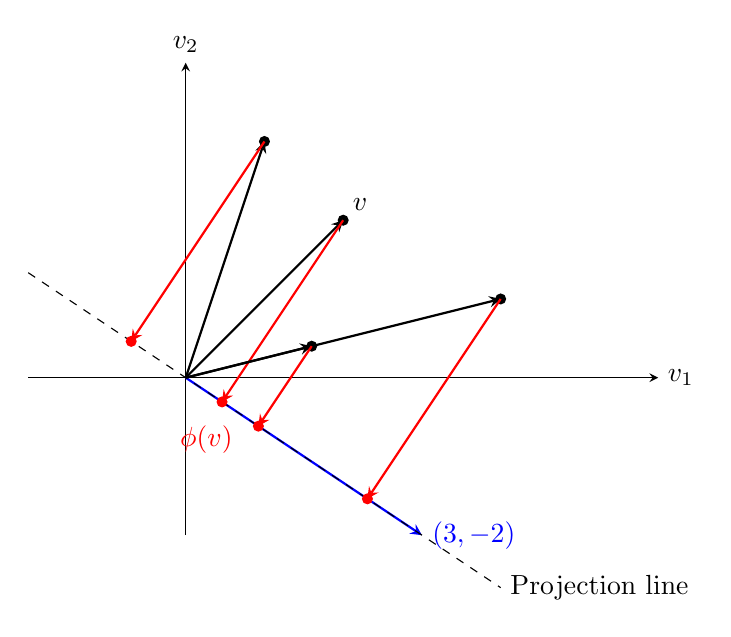
\begin{tikzpicture}[scale=2, >=stealth, vector/.style={thick,->}]
	
	% Draw the coordinate axes
	\draw[->] (-1,0) -- (3,0) node[right] {$v_1$};
	\draw[->] (0,-1) -- (0,2) node[above] {$v_2$};
	
	% Draw the projection line (scalar line) corresponding to the transformation direction
	\draw[vector, blue] (0,0) -- (1.5,-1) node[right] {$(3,-2)$}; % Vector indicating transformation direction
	\draw[dashed, thin] (-1,0.6667) -- (2,-1.3333) node[right] {Projection line};
	
	% Draw vectors and their projections
	\foreach \x/\y in {1/1, 0.5/1.5, 2/0.5, 0.8/0.2}{
		\pgfmathsetmacro{\t}{(3*\x - 2*\y)/(3*3 + 2*2)}
		\pgfmathsetmacro{\px}{3*\t}
		\pgfmathsetmacro{\py}{-2*\t}
		\draw[vector] (0,0) -- (\x,\y);
		\fill (\x,\y) circle(1pt);
		\draw[vector, red] (\x,\y) -- (\px,\py);
		\fill[red] (\px,\py) circle(1pt);
	}
	
	% Labeling a typical vector and its projection
	\node at (1,1) [above right] {$v$};
	\node at (0.36, -0.24) [below left, red] {$\phi(v)$};
	
\end{tikzpicture}

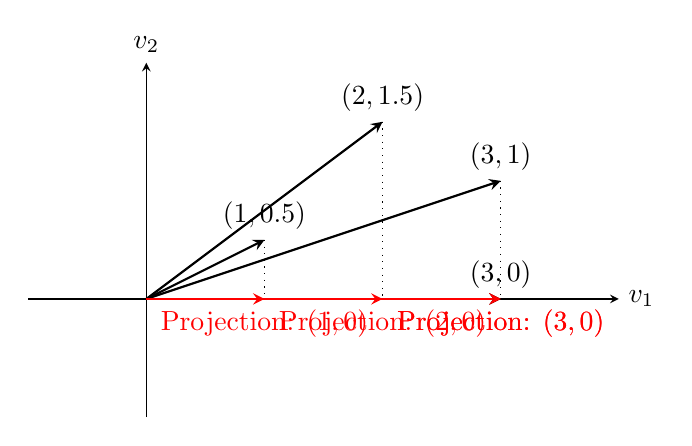
\begin{tikzpicture}[scale=1.5, >=stealth]
	% Draw the coordinate axes
	\draw[->] (-1,0) -- (4,0) node[right] {$v_1$};
	\draw[->] (0,-1) -- (0,2) node[above] {$v_2$};
	
	% Draw a few vectors and their projections onto the x-axis
	\foreach \x/\y in {3/1, 2/1.5, 1/0.5, 3/0} {
		% Original vector
		\draw[thick,->] (0,0) -- (\x,\y) node[at end, above] {$(\x,\y)$};
		% Projection onto the x-axis
		\draw[thick,->, red] (0,0) -- (\x,0) node[at end, below] {Projection: $(\x,0)$};
		% Connection line to projection (dotted)
		\draw[dotted] (\x,\y) -- (\x,0);
	}
\end{tikzpicture}

\begin{tikzcd}[row sep=huge, column sep=huge]
	V \arrow[r, "T"] \arrow[d, "(\cdot)^*", swap] & 
	W \arrow[d, "(\cdot)^*"] \\
	V^* \arrow[r, "T^*", swap] & 
	W^* \\
	V^{**} \arrow[r, "T^{**}"] \arrow[u, "(\cdot)^*", swap] & 
	W^{**} \arrow[u, "(\cdot)^*"]
\end{tikzcd}
\begin{definition}[Vector Space and Dual Space]
\ \begin{itemize}
	\item Let $V$ be a finite-dimensional \emph{vector space} over field $\mathbb{K}$. That is, $V=K^n$.
	\item The \emph{dual space} $V^*$ of $V$ consists of all linear functionals on $V$. That is, $$V^* = \{\phi: V \rightarrow \mathbb{R} \mid \phi \text{ is linear}\}.$$
\end{itemize}
\end{definition}

\begin{definition}[Double Dual Space]
	The \emph{double dual space} $V^{**}$ of a vector space $V$ is defined as the dual of the dual space, i.e., $V^{**} = (V^*)^*$. For each $\psi \in V^{**}$, $\psi$ is a functional acting on elements of $V^*$.
\end{definition}

\section*{Natural Isomorphism Between $V$ and $V^{**}$}
\begin{theorem}[Canonical Isomorphism]
	For every finite-dimensional vector space $V$, there is a canonical isomorphism $\eta_V: V \rightarrow V^{**}$ defined by
	\[
	\eta_V(v)(\phi) = \phi(v),
	\]
	for every
$v \in V$ and $\phi \in V^*$. This map is a natural isomorphism, meaning it commutes with all linear transformations.
\end{theorem}
\begin{definition}[Induced Map on Dual and Double Dual Spaces]
	For a linear transformation $T: V \rightarrow W$ between vector spaces, the induced map on the dual space, $T^*: W^* \rightarrow V^*$, is defined by \[
	T^*(\phi)=\phi\circ T, 
	\] where $\phi \in W^*$. Similarly, the induced map on the double dual space, $T^{**}: V^{**} \rightarrow W^{**}$, is defined by \[
	T^{**}(\psi)=\psi\circ T^*,
	\] where $\psi \in V^{**}$.
\end{definition}
\section{Example: Application in $\mathbb{R}^2$}
\begin{example}[Matrix Transformation and Double Dual]
	Consider the vector space $V = \mathbb{R}^2$, and let $T: \mathbb{R}^2 \rightarrow \mathbb{R}^2$ be represented by the matrix
	\[
	A=\begin{bmatrix}
		1 & 2 \\ 3 & 4
	\end{bmatrix}
	\] We compute the induced maps $T^*$ and $T^{**}$ and verify the natural transformation property with $\eta_V$.
	
	\textbf{Action of $T$ and $\eta_V$:}
	If $\mathbf{v} = (1, 1)$, then \[
	T(\textbf{v})=A\begin{bmatrix}
		1 \\ 1
	\end{bmatrix} = \begin{bmatrix}
	3 \\ 7
\end{bmatrix}.
	\] The action of $\eta_{\mathbb{R}^2}$ and $\phi$ defined by $\phi(\mathbf{v}) = 3v_1 - 2v_2$ gives \[
	\eta_{\R^2}((1,1))(\phi)=1\quad\text{and}\quad\eta_{\R^2}((3,7))(\phi)=3\times 3-2\times 7=-5.
	\] \textbf{Verification of Commutativity:}
	To confirm the natural transformation property, we need to show \[
	T^{**}(\eta_{\R^2}(\textbf{v}))=\eta_{\R^2}(T(\textbf{v})).
	\]
	For $\mathbf{v} = (1, 1)$, the calculations show that both sides of the equation represent consistent transformations via the isomorphism $\eta_{\mathbb{R}^2}$, proving the natural transformation.
\end{example}
\newpage
\begin{example}
\ \begin{itemize}
	\item[] \textbf{[ Category ]}
	\begin{enumerate}
		\item \textbf{Category of Finite Vector Spaces} ($\mathsf{FinVect}_K$)
		\begin{itemize}
			\item \textbf{Objects}: 
			\begin{itemize}
				\item Vector space $V=K^n$ over a field $K$
				\item Dual Space $V^*=\set{\phi\in K^{V}:\phi\ \text{is linear transformation}}$.
			\end{itemize}
			\item \textbf{Morphisms}:  
			\begin{itemize}
				\item Linear Transformation $T:V(=K^n)\to W(=K^m)$
				\item Dual Transformation $T^*:W^*\to V^*$ defined by \[
				T^*f:=f\circ T\quad\text{for all}\quad f\in W*.
				\] Sometimes we denote $V^*:=\mathcal{L}(V,K)$. Note that \begin{itemize}
					\item $(T^*f)\textbf{v}=f(T\textbf{v})$ for all $\textbf{v}\in V$;
					\item $f\in W^*\implies T^*f\in V^*$;
					\item $T^*$ is linear.
				\end{itemize}
			\end{itemize}
		\end{itemize}
	\end{enumerate}
	\item[] \textbf{[ Functor ]}
	\begin{enumerate}
		\item \textbf{Dual Space Functor} ($\mathcal{D}:\mathsf{FinVect}_K\to\mathsf{FinVect}_K$)
		\begin{itemize}
			\item \textbf{On Objects}: \[
			V\mapsto V^*=\mathcal{D}(V)
			\] Maps a vector space $V$ to the dual space $V^*$, which  which consists of all linear functionals from $V$ to $K$.
			\item \textbf{On Morphisms}:\[
			T\mapsto T^*=\mathcal{D}(T)
			\]
		\end{itemize}
	\end{enumerate}
	\item \textbf{[ Natural Transformation: Determinant ]} The determinant \[
	\text{det}_R:GL_n(R)\to R^{\times}
	\] is a natural transformation between two functors, $\mathbf{GL}_n$ and $\mathbf{U}$.
\end{itemize}
\end{example}
